\chapter{Introdución}
\label{chap:introducion}

\lettrine{E}{n} este capítulo, exploraremos la motivación detrás de este trabajo, proporcionando un análisis detallado de los propósitos establecidos al inicio del proyecto y, por último, se presentarán los apartados que compondrán la memoria.



\section{Motivación}
\label{sec:motivacion}
Los bosques son una parte fundamental de nuestra vida cotidiana. Proporcionan hábitats para muchas especies, regulan el ciclo del agua, ayudan a moderar el cambio climático al absorber dióxido de carbono y proporcionan importantes recursos naturales como  madera y  alimentos.

Sin embargo, como podemos ver en la figura \ref{fig:drivers of forest lost} obtenida en la web de \textit{Our World in Data} \cite{owidforestsanddeforestation} la deforestación los esta destruyendo. Entre los motivos para esto esta la creación de nuevos terrenos edificables o las substitución del cultivo como esta ocurriendo en indonesia con las palma aceitera. Si pudiéramos tener una lista de  árboles en diferentes bosques, podríamos identificar estos eventos y buscar soluciones para mitigar las consecuencias de la pérdida de estos entornos.

En la actualidad, la realización de inventarios y  de árboles se lleva a cabo de manera manual, lo que implica una inversión de mucho tiempo y recursos humanos considerables. Esta tarea se vuelve aún más desafiante en países donde la cobertura forestal puede representar hasta el 67\% del territorio, como es el caso de Suecia \cite{sweeden}.

En este contexto, entraria en juego la tecnología LiDAR, que aprovechando las nubes de puntos obtenidas meidante sensores equipados en vehículos aéreos no tripulados (UAV) y mediante la aplicación de algoritmos avanzados y técnicas , como el aprendizaje profundo, nos permitiría automatizar el proceso de inventariado de los bosques. Este enfoque ha ganado  bastante popularidad en los últimos años, impulsado por avances en los sensores LiDAR y la creciente accesibilidad a UAVs.

La adopción de esta tecnología y la automatización en la detección de árboles en nubes de puntos prometen revolucionar la forma en que abordamos la gestión y conservación de los bosques. Al agilizar y perfeccionar el proceso de inventario, podemos detectar y responder de manera más efectiva a eventos como la deforestación.

\begin{figure}[h]
\centering
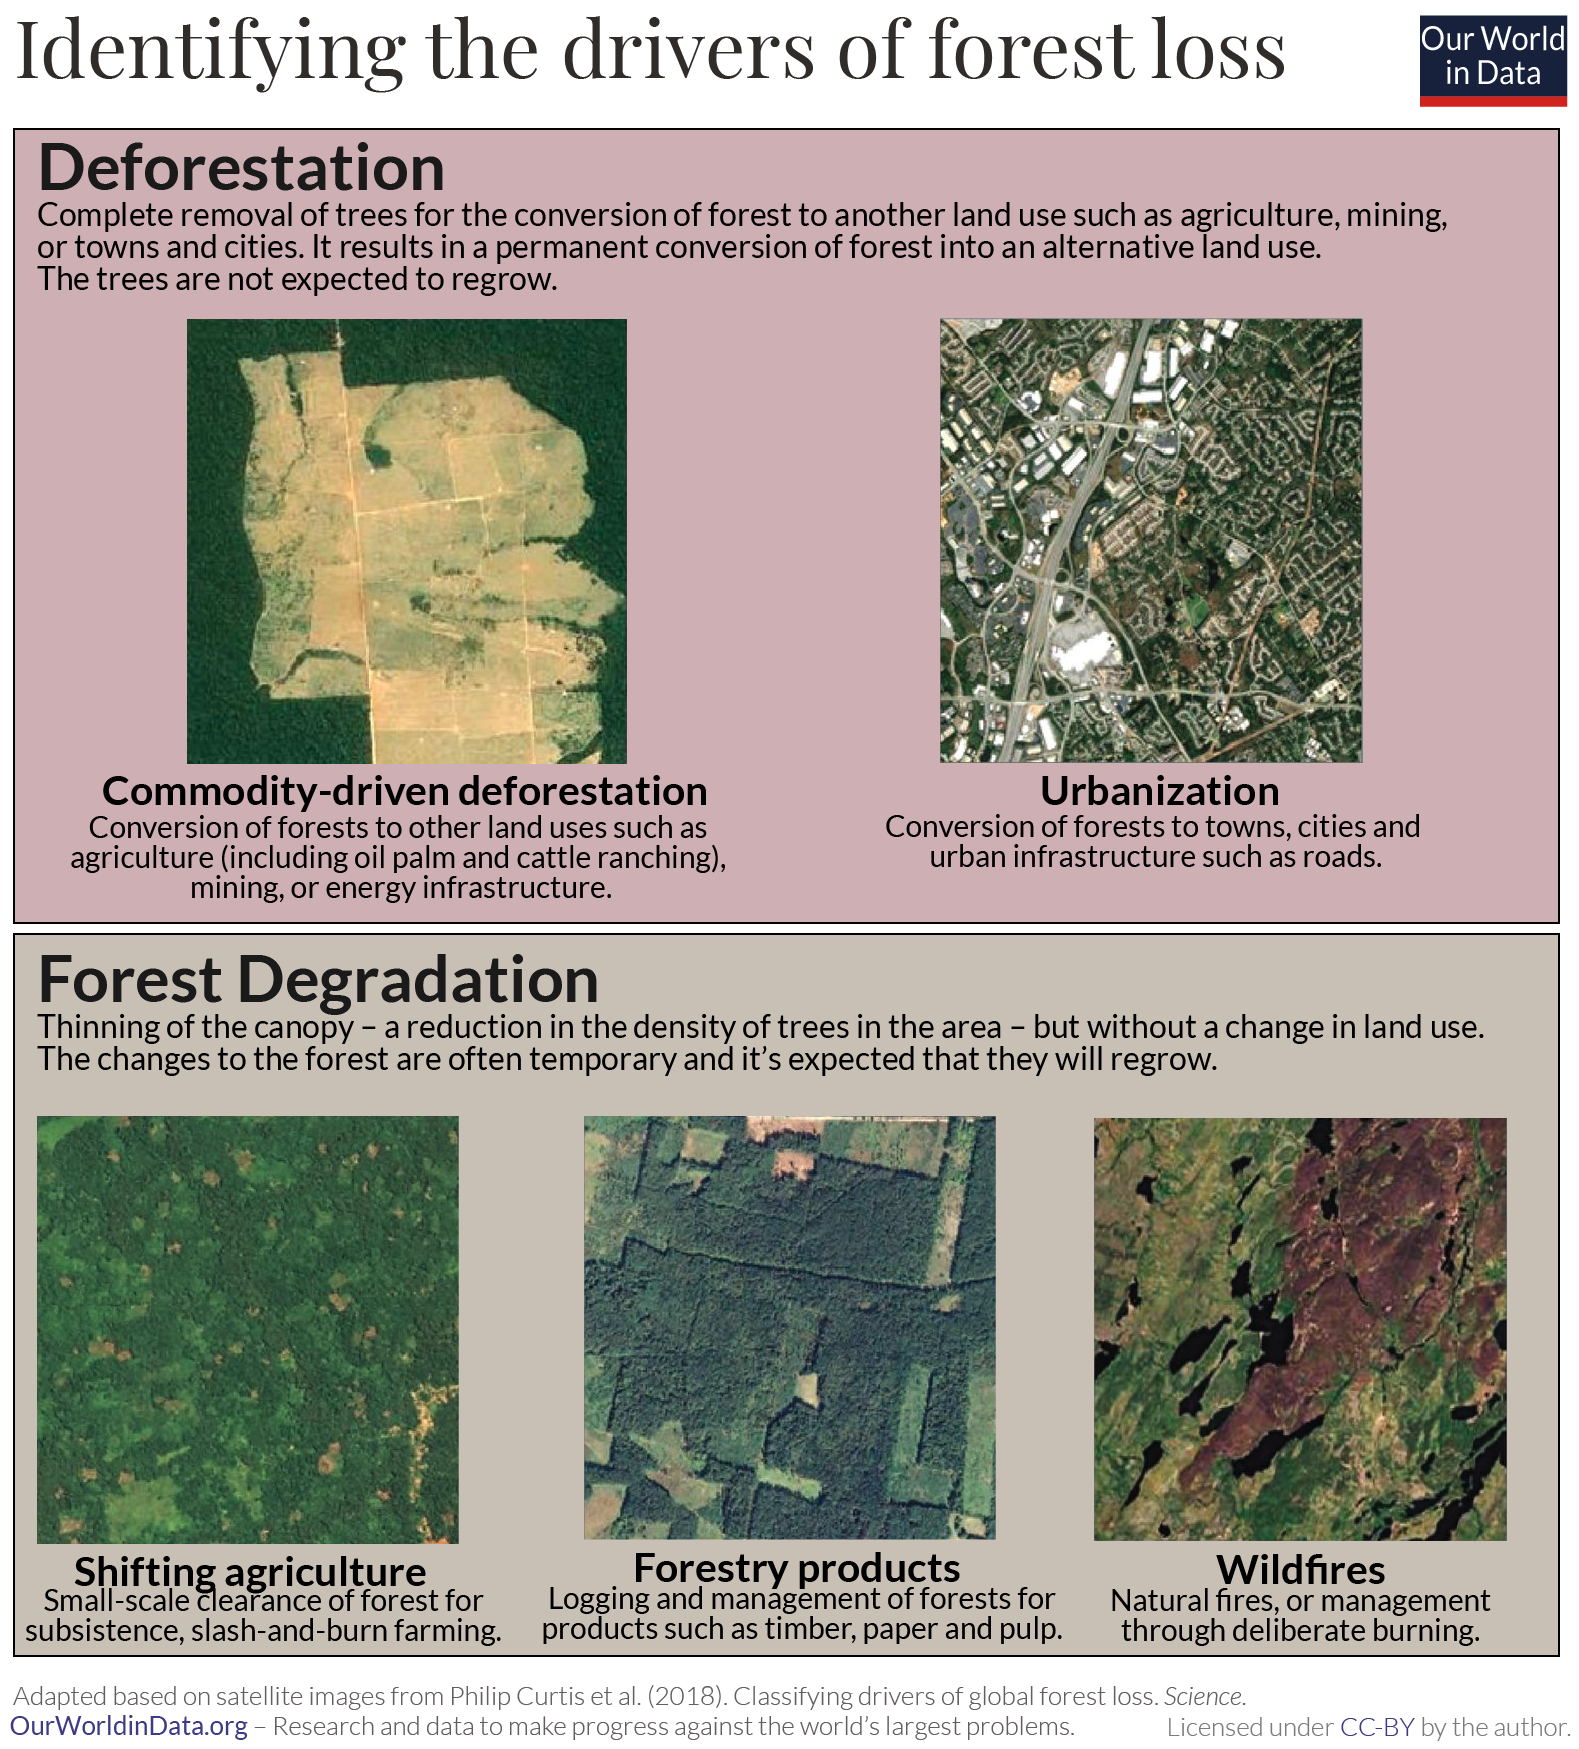
\includegraphics[width=8cm]{imaxes/Identifying-drivers-of-forest-loss.png}
\caption{Gráfico con las principales causas de la perdida de bosques}
\label{fig:drivers of forest lost}
\end{figure}

\section{Objetivos}
\label{sec:Objetivos}

El propósito central de este estudio es llevar a cabo la detección y el conteo de árboles en nubes de puntos LiDAR. La detección se realizará mediante la implementación de algoritmos basados en características geométricas.Estos objetivos principales los podemos desglosar en los siguientes :

\begin{itemize}
    \item Comprender el funcionamiento de la tecnología LiDAR y los datos obtenidos con ella como las nubes de puntos para poder procesar la información en ellas.
    \item Buscar conjuntos de datos adecuados, con una cierta densidad de puntos, y aprender a utilizar las principales herramientas para el procesamiento y la visualización de nubes de puntos.
    \item Investigar las librerías para procesado de nubes de puntos en python.
    \item Probar diferentes algoritmos y aproximaciones para detectar arboles y estudiar su precisión.
    \item Analizar y Comparar los resultados obtenidos.
\end{itemize}

\section{Apartados de la memoria}
\label{sec:apartados}
La memoria está conformada por los siguientes apartados:
\begin{enumerate}
    \item \textbf{Introducción} : Se introduciremos el proyecto y las motivaciones para llevarlo a cabo. Además, se expondrán los objetivos que perseguiremos durante su desarrollo.

    \item \textbf{Fundamentos Teóricos y Tecnológicos} : Se expondrá una breve introducción a la tecnología LiDAR y la forma en que se guardan los datos obtenidos de esta.
    
    \item \textbf{Metodología} : Comentaremos la metodología elegida para llevar a cabo el trabajo y el por qué de su elección.
    
    \item \textbf{Planificación} : Abordaremos la planificación llevada a cabo para el desarrollo de este proyecto, así como el costo que conllevó su ejecución.
    
    \item \textbf{Detección de árboles basada en estratos} : Se explicará la implementación del algoritmo para la detección de los árboles.
    
    \item \textbf{Análisis de Resultados} : Se probará el algoritmo en diferentes partes del conjunto de datos de Luxemburgo y se estudiarán y analizarán los resultados obtenidos.
    
    \item \textbf{Conclusiones y Trabajo Futuro} : En el capítulo final se presentarán las conclusiones obtenidas en el análisis de los datos y se formularán posibles mejoras que podrían llevarse a cabo en el futuro.


\end{enumerate}

